% Neural network diagram
% Made with Xematics. Positions are in px (1 px = 0.75 pt), as in the SVG export.
\documentclass[tikz, border=4pt]{standalone}
\definecolor{xm1}{HTML}{FFFFFF}
\definecolor{xm2}{HTML}{F5F5F5}
\definecolor{xm3}{HTML}{000000}
\definecolor{xm4}{HTML}{F1F1F1}
\definecolor{xm5}{HTML}{A6A6A6}
\definecolor{xm6}{HTML}{D9D9D9}
\definecolor{xm7}{HTML}{CCCCCC}
\definecolor{xm8}{HTML}{595959}
\definecolor{xm9}{HTML}{4D4D4D}
\begin{document}
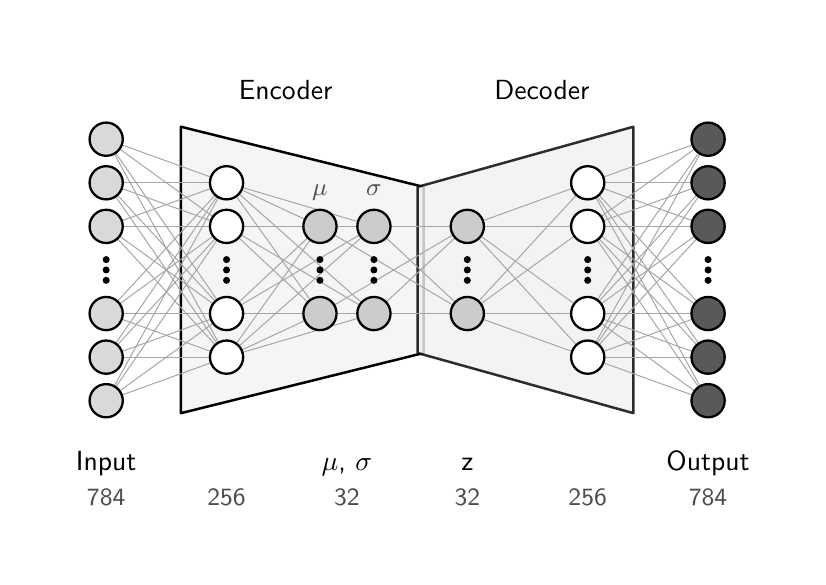
\begin{tikzpicture}[x=0.75pt, y=-0.75pt]
  \tikzset{
    xm funnel fsyzdz/.style={fill=xm2, draw=xm3, line width=0.9pt, line join=round},
    xm funnel 14qqp3/.style={fill=xm4, draw=xm3, line width=0.9pt, opacity=0.82, line join=round},
    xm edge 1rgo9bh/.style={draw=xm5, line width=0.36pt},
    xm node 1nsv9ws/.style={fill=xm6, draw=xm3, line width=0.83pt},
    xm circle 1myn5ok/.style={fill=xm3},
    xm node 1mv6k0h/.style={fill=xm1, draw=xm3, line width=0.83pt},
    xm node 1nzlthn/.style={fill=xm7, draw=xm3, line width=0.83pt},
    xm node 1o6cd2i/.style={fill=xm8, draw=xm3, line width=0.83pt},
    xm text xm9/.style={text=xm9, inner sep=0},
    xm text xm3/.style={text=xm3, inner sep=0},
  }
  \fill[xm1] (0,0) rectangle (371.07,254.98);
  % Diagram
  \path[xm funnel fsyzdz] (73.82,47.73) -- (190.82,76.73) -- (190.82,156.73) -- (73.82,185.73) -- cycle;
  \path[xm funnel 14qqp3] (187.82,76.73) -- (291.82,47.73) -- (291.82,185.73) -- (187.82,156.73) -- cycle;
  \path[xm edge 1rgo9bh] (45.34,56.45) -- (88.3,72.01);
  \path[xm edge 1rgo9bh] (44.3,58.42) -- (89.34,91.04);
  \path[xm edge 1rgo9bh] (42.37,60.31) -- (91.28,131.15);
  \path[xm edge 1rgo9bh] (41.69,60.73) -- (91.95,151.73);
  \path[xm edge 1rgo9bh] (45.82,74.73) -- (87.82,74.73);
  \path[xm edge 1rgo9bh] (45.34,77.45) -- (88.3,93.01);
  \path[xm edge 1rgo9bh] (43.24,80.62) -- (90.4,131.84);
  \path[xm edge 1rgo9bh] (42.37,81.31) -- (91.28,152.15);
  \path[xm edge 1rgo9bh] (45.34,93.01) -- (88.3,77.45);
  \path[xm edge 1rgo9bh] (45.82,95.73) -- (87.82,95.73);
  \path[xm edge 1rgo9bh] (44.3,100.42) -- (89.34,133.04);
  \path[xm edge 1rgo9bh] (43.24,101.62) -- (90.4,152.84);
  \path[xm edge 1rgo9bh] (43.24,131.84) -- (90.4,80.62);
  \path[xm edge 1rgo9bh] (44.3,133.04) -- (89.34,100.42);
  \path[xm edge 1rgo9bh] (45.82,137.73) -- (87.82,137.73);
  \path[xm edge 1rgo9bh] (45.34,140.45) -- (88.3,156.01);
  \path[xm edge 1rgo9bh] (42.37,152.15) -- (91.28,81.31);
  \path[xm edge 1rgo9bh] (43.24,152.84) -- (90.4,101.62);
  \path[xm edge 1rgo9bh] (45.34,156.01) -- (88.3,140.45);
  \path[xm edge 1rgo9bh] (45.82,158.73) -- (87.82,158.73);
  \path[xm edge 1rgo9bh] (41.69,172.73) -- (91.95,81.73);
  \path[xm edge 1rgo9bh] (42.37,173.15) -- (91.28,102.31);
  \path[xm edge 1rgo9bh] (44.3,175.04) -- (89.34,142.42);
  \path[xm edge 1rgo9bh] (45.34,177.01) -- (88.3,161.45);
  \path[xm edge 1rgo9bh] (103.07,78.11) -- (133.57,92.35);
  \path[xm edge 1rgo9bh] (100.47,81.24) -- (136.17,131.22);
  \path[xm edge 1rgo9bh] (103.49,77) -- (159.15,93.46);
  \path[xm edge 1rgo9bh] (101.81,80.04) -- (160.84,132.42);
  \path[xm edge 1rgo9bh] (103.82,95.73) -- (132.82,95.73);
  \path[xm edge 1rgo9bh] (101.67,101.19) -- (134.97,132.27);
  \path[xm edge 1rgo9bh] (103.82,95.73) -- (158.82,95.73);
  \path[xm edge 1rgo9bh] (102.71,99.8) -- (159.94,133.66);
  \path[xm edge 1rgo9bh] (101.67,132.27) -- (134.97,101.19);
  \path[xm edge 1rgo9bh] (103.82,137.73) -- (132.82,137.73);
  \path[xm edge 1rgo9bh] (102.71,133.66) -- (159.94,99.8);
  \path[xm edge 1rgo9bh] (103.82,137.73) -- (158.82,137.73);
  \path[xm edge 1rgo9bh] (100.47,152.22) -- (136.17,102.24);
  \path[xm edge 1rgo9bh] (103.07,155.35) -- (133.57,141.11);
  \path[xm edge 1rgo9bh] (101.81,153.42) -- (160.84,101.04);
  \path[xm edge 1rgo9bh] (103.49,156.46) -- (159.15,140);
  \path[xm edge 1rgo9bh] (148.82,95.73) -- (203.82,95.73);
  \path[xm edge 1rgo9bh] (147.71,99.8) -- (204.94,133.66);
  \path[xm edge 1rgo9bh] (147.71,133.66) -- (204.94,99.8);
  \path[xm edge 1rgo9bh] (148.82,137.73) -- (203.82,137.73);
  \path[xm edge 1rgo9bh] (174.82,95.73) -- (203.82,95.73);
  \path[xm edge 1rgo9bh] (172.67,101.19) -- (205.97,132.27);
  \path[xm edge 1rgo9bh] (172.67,132.27) -- (205.97,101.19);
  \path[xm edge 1rgo9bh] (174.82,137.73) -- (203.82,137.73);
  \path[xm edge 1rgo9bh] (219.34,93.01) -- (262.3,77.45);
  \path[xm edge 1rgo9bh] (219.82,95.73) -- (261.82,95.73);
  \path[xm edge 1rgo9bh] (218.3,100.42) -- (263.34,133.04);
  \path[xm edge 1rgo9bh] (217.24,101.62) -- (264.4,152.84);
  \path[xm edge 1rgo9bh] (217.24,131.84) -- (264.4,80.62);
  \path[xm edge 1rgo9bh] (218.3,133.04) -- (263.34,100.42);
  \path[xm edge 1rgo9bh] (219.82,137.73) -- (261.82,137.73);
  \path[xm edge 1rgo9bh] (219.34,140.45) -- (262.3,156.01);
  \path[xm edge 1rgo9bh] (277.34,72.01) -- (320.3,56.45);
  \path[xm edge 1rgo9bh] (277.82,74.73) -- (319.82,74.73);
  \path[xm edge 1rgo9bh] (277.34,77.45) -- (320.3,93.01);
  \path[xm edge 1rgo9bh] (275.24,80.62) -- (322.4,131.84);
  \path[xm edge 1rgo9bh] (274.37,81.31) -- (323.28,152.15);
  \path[xm edge 1rgo9bh] (273.69,81.73) -- (323.95,172.73);
  \path[xm edge 1rgo9bh] (276.3,91.04) -- (321.34,58.42);
  \path[xm edge 1rgo9bh] (277.34,93.01) -- (320.3,77.45);
  \path[xm edge 1rgo9bh] (277.82,95.73) -- (319.82,95.73);
  \path[xm edge 1rgo9bh] (276.3,100.42) -- (321.34,133.04);
  \path[xm edge 1rgo9bh] (275.24,101.62) -- (322.4,152.84);
  \path[xm edge 1rgo9bh] (274.37,102.31) -- (323.28,173.15);
  \path[xm edge 1rgo9bh] (274.37,131.15) -- (323.28,60.31);
  \path[xm edge 1rgo9bh] (275.24,131.84) -- (322.4,80.62);
  \path[xm edge 1rgo9bh] (276.3,133.04) -- (321.34,100.42);
  \path[xm edge 1rgo9bh] (277.82,137.73) -- (319.82,137.73);
  \path[xm edge 1rgo9bh] (277.34,140.45) -- (320.3,156.01);
  \path[xm edge 1rgo9bh] (276.3,142.42) -- (321.34,175.04);
  \path[xm edge 1rgo9bh] (273.69,151.73) -- (323.95,60.73);
  \path[xm edge 1rgo9bh] (274.37,152.15) -- (323.28,81.31);
  \path[xm edge 1rgo9bh] (275.24,152.84) -- (322.4,101.62);
  \path[xm edge 1rgo9bh] (277.34,156.01) -- (320.3,140.45);
  \path[xm edge 1rgo9bh] (277.82,158.73) -- (319.82,158.73);
  \path[xm edge 1rgo9bh] (277.34,161.45) -- (320.3,177.01);
  \path[xm node 1nsv9ws] (37.82,53.73) circle[radius=8];
  \path[xm node 1nsv9ws] (37.82,74.73) circle[radius=8];
  \path[xm node 1nsv9ws] (37.82,95.73) circle[radius=8];
  \path[xm circle 1myn5ok] (37.82,111.73) circle[radius=1.7];
  \path[xm circle 1myn5ok] (37.82,116.73) circle[radius=1.7];
  \path[xm circle 1myn5ok] (37.82,121.73) circle[radius=1.7];
  \path[xm node 1nsv9ws] (37.82,137.73) circle[radius=8];
  \path[xm node 1nsv9ws] (37.82,158.73) circle[radius=8];
  \path[xm node 1nsv9ws] (37.82,179.73) circle[radius=8];
  \path[xm node 1mv6k0h] (95.82,74.73) circle[radius=8];
  \path[xm node 1mv6k0h] (95.82,95.73) circle[radius=8];
  \path[xm circle 1myn5ok] (95.82,111.73) circle[radius=1.7];
  \path[xm circle 1myn5ok] (95.82,116.73) circle[radius=1.7];
  \path[xm circle 1myn5ok] (95.82,121.73) circle[radius=1.7];
  \path[xm node 1mv6k0h] (95.82,137.73) circle[radius=8];
  \path[xm node 1mv6k0h] (95.82,158.73) circle[radius=8];
  \path[xm node 1nzlthn] (140.82,95.73) circle[radius=8];
  \path[xm circle 1myn5ok] (140.82,111.73) circle[radius=1.7];
  \path[xm circle 1myn5ok] (140.82,116.73) circle[radius=1.7];
  \path[xm circle 1myn5ok] (140.82,121.73) circle[radius=1.7];
  \path[xm node 1nzlthn] (140.82,137.73) circle[radius=8];
  \path[xm node 1nzlthn] (166.82,95.73) circle[radius=8];
  \path[xm circle 1myn5ok] (166.82,111.73) circle[radius=1.7];
  \path[xm circle 1myn5ok] (166.82,116.73) circle[radius=1.7];
  \path[xm circle 1myn5ok] (166.82,121.73) circle[radius=1.7];
  \path[xm node 1nzlthn] (166.82,137.73) circle[radius=8];
  \path[xm node 1nzlthn] (211.82,95.73) circle[radius=8];
  \path[xm circle 1myn5ok] (211.82,111.73) circle[radius=1.7];
  \path[xm circle 1myn5ok] (211.82,116.73) circle[radius=1.7];
  \path[xm circle 1myn5ok] (211.82,121.73) circle[radius=1.7];
  \path[xm node 1nzlthn] (211.82,137.73) circle[radius=8];
  \path[xm node 1mv6k0h] (269.82,74.73) circle[radius=8];
  \path[xm node 1mv6k0h] (269.82,95.73) circle[radius=8];
  \path[xm circle 1myn5ok] (269.82,111.73) circle[radius=1.7];
  \path[xm circle 1myn5ok] (269.82,116.73) circle[radius=1.7];
  \path[xm circle 1myn5ok] (269.82,121.73) circle[radius=1.7];
  \path[xm node 1mv6k0h] (269.82,137.73) circle[radius=8];
  \path[xm node 1mv6k0h] (269.82,158.73) circle[radius=8];
  \path[xm node 1o6cd2i] (327.82,53.73) circle[radius=8];
  \path[xm node 1o6cd2i] (327.82,74.73) circle[radius=8];
  \path[xm node 1o6cd2i] (327.82,95.73) circle[radius=8];
  \path[xm circle 1myn5ok] (327.82,111.73) circle[radius=1.7];
  \path[xm circle 1myn5ok] (327.82,116.73) circle[radius=1.7];
  \path[xm circle 1myn5ok] (327.82,121.73) circle[radius=1.7];
  \path[xm node 1o6cd2i] (327.82,137.73) circle[radius=8];
  \path[xm node 1o6cd2i] (327.82,158.73) circle[radius=8];
  \path[xm node 1o6cd2i] (327.82,179.73) circle[radius=8];
  \node[xm text xm9, font=\sffamily\fontsize{9}{10.8}\selectfont, anchor=base] at (140.82,80.73) {\ensuremath{\mu}};
  \node[xm text xm9, font=\sffamily\fontsize{9}{10.8}\selectfont, anchor=base] at (166.82,80.73) {\ensuremath{\sigma}};
  \node[xm text xm3, font=\sffamily\fontsize{9.75}{11.7}\selectfont, anchor=base] at (124.32,34.59) {Encoder};
  \node[xm text xm3, font=\sffamily\fontsize{9.75}{11.7}\selectfont, anchor=base] at (247.82,34.59) {Decoder};
  \node[xm text xm3, font=\sffamily\fontsize{9.75}{11.7}\selectfont, anchor=base] at (37.82,213.32) {Input};
  \node[xm text xm9, font=\sffamily\fontsize{9}{10.8}\selectfont, anchor=base] at (37.82,230.08) {784};
  \node[xm text xm9, font=\sffamily\fontsize{9}{10.8}\selectfont, anchor=base] at (95.82,230.08) {256};
  \node[xm text xm3, font=\sffamily\fontsize{9.75}{11.7}\selectfont, anchor=base] at (153.82,213.32) {\ensuremath{\mu}, \ensuremath{\sigma}};
  \node[xm text xm9, font=\sffamily\fontsize{9}{10.8}\selectfont, anchor=base] at (153.82,230.08) {32};
  \node[xm text xm3, font=\sffamily\fontsize{9.75}{11.7}\selectfont, anchor=base] at (211.82,213.32) {z};
  \node[xm text xm9, font=\sffamily\fontsize{9}{10.8}\selectfont, anchor=base] at (211.82,230.08) {32};
  \node[xm text xm9, font=\sffamily\fontsize{9}{10.8}\selectfont, anchor=base] at (269.82,230.08) {256};
  \node[xm text xm3, font=\sffamily\fontsize{9.75}{11.7}\selectfont, anchor=base] at (327.82,213.32) {Output};
  \node[xm text xm9, font=\sffamily\fontsize{9}{10.8}\selectfont, anchor=base] at (327.82,230.08) {784};
\end{tikzpicture}
\end{document}
